\documentclass[12pt]{article}
\usepackage{geometry}                % See geometry.pdf to learn the layout options. There are lots.
\geometry{letterpaper}                   % ... or a4paper or a5paper or ... 
%\geometry{landscape}                % Activate for for rotated page geometry
\usepackage[parfill]{parskip}    % Activate to begin paragraphs with an empty line rather than an indent
\usepackage{daves,fancyhdr,natbib,graphicx,dcolumn,amsmath,lastpage,url}
\usepackage{amsmath,amssymb,epstopdf,longtable}
\usepackage{paralist} 
\DeclareGraphicsRule{.tif}{png}{.png}{`convert #1 `dirname #1`/`basename #1 .tif`.png}
\pagestyle{fancy}
\lhead{CE 3372 -- Water Systems Design}
\rhead{SPRING 2025}
\lfoot{EXERCISE 3}
\cfoot{}
\rfoot{Page \thepage\ of \pageref{LastPage}}
\renewcommand\headrulewidth{0pt}

\begin{document}
\begin{center}
{\textbf{{ CE 3372 -- Water Systems Design} \\ {Demand Estimation} \\ {Exercise Set 3}}}
\end{center}

\section*{\small{Exercise}} 
\begin{enumerate}
%\item %Figure \ref{fig:newport-base-map} is a map of a proposed subdivision.  Each lot will house an executive home.  

%\begin{figure}[h!] %  figure placement: here, top, bottom, or page
%\centering
%   \includegraphics[width=6in]{newport-base-map.jpg}
%   \caption{Newport Subdivision Proposed Development}
%   \label{fig:newport-base-map} 
%\end{figure}
%\clearpage



%Figure \ref{fig:newport-pipe-layout} is a skeletonized layout for a network model of the water distribution system.
%Each small black circle is a distribution node that serves several lots.
%Each red circle represents a fire-hydrant location.
%Water is supplied by the lift station depicted in the lower left corner of the drawing.   
%
%\begin{enumerate}[a)]
%\item Estimate the average daily demand (ADD) for the entire distribution system using San Marcos, Texas water system design guidelines.
%\item Estimate the maximum daily demand (MDD) for the entire distribution system using San Marcos, Texas water system design guidelines.
%\item Estimate the maximum daily demand (MDD) + fire flow for the entire distribution system using San Marcos, Texas water system design guidelines.
%\item Estimate the peak hourly demand (PHD) for the entire distribution system using San Marcos, Texas water system design guidelines.
%\item Estimate the average daily demand (ADD) for the entire distribution system using Riverside County, CA. water system design guidelines.
%\item Estimate the maximum daily demand (MDD) for the entire distribution system using Riverside County, CA. water system design guidelines.
%\item Estimate the maximum daily demand (MDD) + fire flow for the entire distribution system using Riverside County, CA. water system design guidelines.
%\item Estimate the peak hourly demand (PHD) for the entire distribution system using Riverside County, CA. water system design guidelines.
%\end{enumerate}
%
%\begin{figure}[h!] %  figure placement: here, top, bottom, or page
%\centering
%   \includegraphics[width=6in]{newport-pipe-layout-flat.png}
%   \caption{Newport Subdivision EPANET Model Pipe Layout}
%   \label{fig:newport-pipe-layout} 
%\end{figure}
%\clearpage
\item Figure \ref{fig:water_network_layout} is a layout of a hydraulic network model for the Somewhere USA subdivision.   
The blue line segments are pipes and are labeled (P1, P2, $\dots$).   
The blue circles are nodes and are labeled (N1, N2, $\dots$).
The yellow polygons represent the lots assigned to each node; for example, node N2 supplies the six (6) lots located near the node.
\begin{figure}[ht!] %  figure placement: here, top, bottom, or page
   \centering
   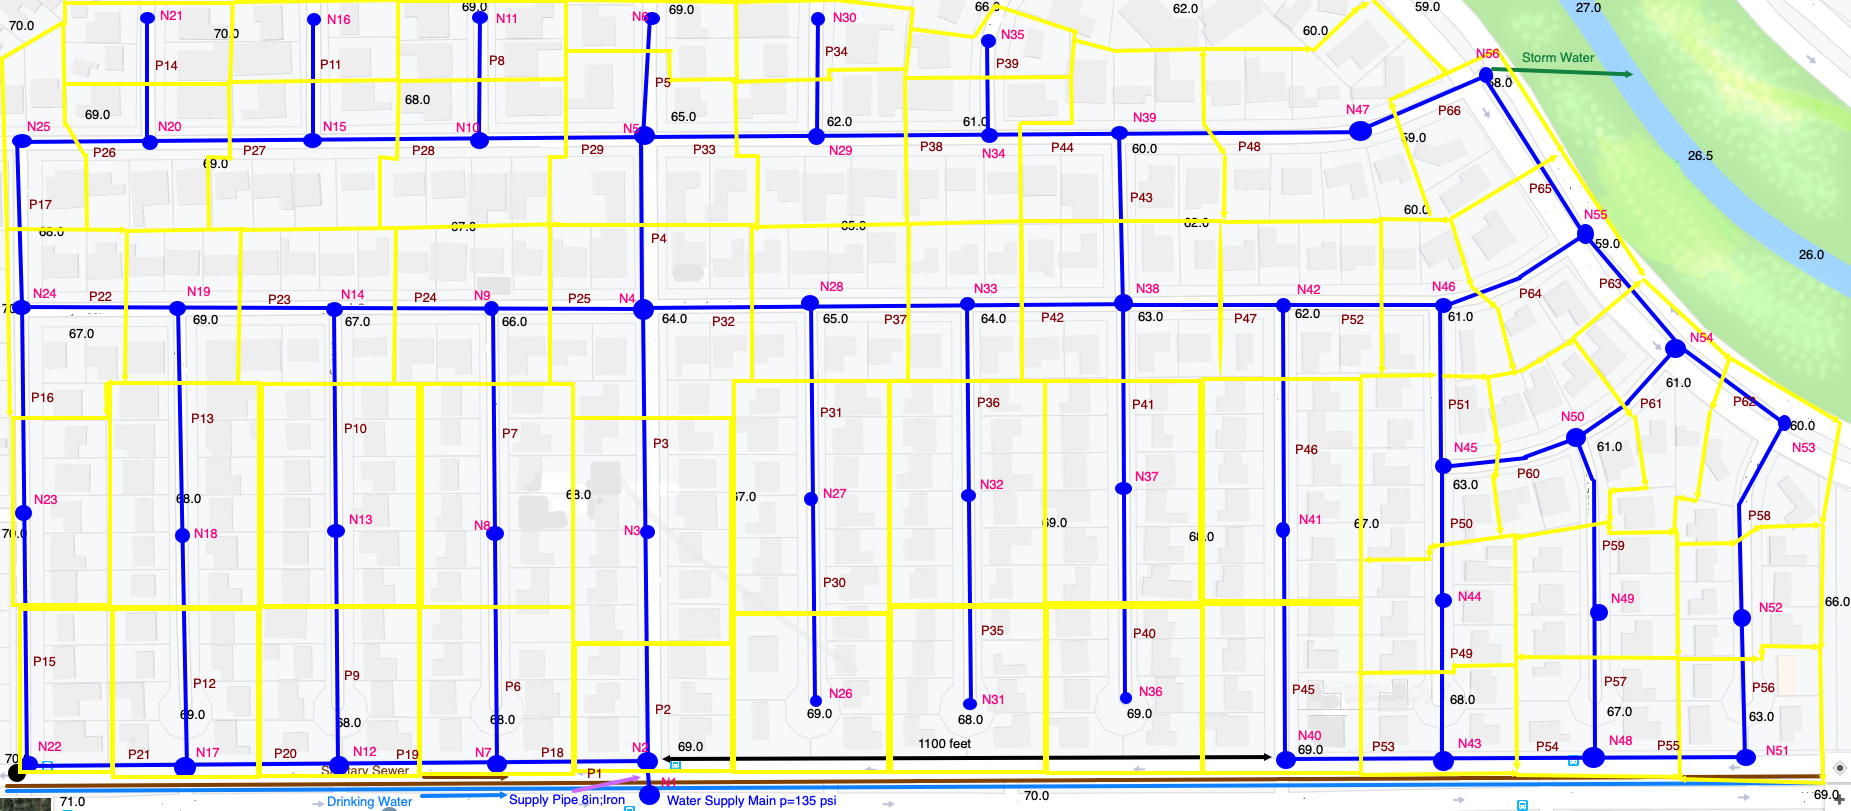
\includegraphics[width=6.5in]{SomewhereClipNodes.jpg} 
   \caption{Hydraulic Model Network for Somewhere USA}
   \label{fig:water_network_layout}
\end{figure}
\begin{enumerate}[a)]
\item Determine the number of lots served by each node, these will constitute the by-node service unit equivalent (SUE).
\item Estimate the average daily demand (ADD), by-node, for distribution system using San Marcos, Texas water system design guidelines.
\item Estimate the maximum daily demand (MDD), by-node, for the distribution system using San Marcos, Texas water system design guidelines.
\item Estimate the maximum daily demand (MDD) + fire flow, by-node for the distribution system using San Marcos, Texas water system design guidelines.
\item Estimate the peak hourly demand (PHD), by-node, for the distribution system using San Marcos, Texas water system design guidelines.
\end{enumerate}
Use your estimates to produce a completed version of Table \ref{tab:ByNodes}.
Save the table (in a file) -- you will need it later in the design project RP-1.
% Requires the booktabs if the memoir class is not being used
\begin{table}[h!]
   \centering
   \caption{Node Demands for Somewhere USA Distribution System}
   \begin{tabular}{p{1in}p{1in}p{1in}p{1in}p{1in}p{1in}} % Column formatting, @{} suppresses leading/trailing space
Node ID & SUE & ADD & MDD & MDD+Fire & PHD \\
\hline
\hline
N1 & 0 & 0 & 0 & 0 & 0 \\
N2 & 6 & $\dots$& $\dots$&$\dots$& $\dots$ \\
N3 & 11 & $\dots$& $\dots$&$\dots$& $\dots$ \\
N4 & $\dots$ & $\dots$& $\dots$&$\dots$& $\dots$ \\
N5 & $\dots$ & $\dots$& $\dots$&$\dots$& $\dots$ \\
N6 & $\dots$ & $\dots$& $\dots$&$\dots$& $\dots$ \\
N7 & $\dots$ & $\dots$& $\dots$&$\dots$& $\dots$ \\
N8 & $\dots$ & $\dots$& $\dots$&$\dots$& $\dots$ \\
N9 & $\dots$ & $\dots$& $\dots$&$\dots$& $\dots$ \\
N10 & $\dots$ & $\dots$& $\dots$&$\dots$& $\dots$ \\
N11 & $\dots$ & $\dots$& $\dots$&$\dots$& $\dots$ \\
N12 & $\dots$ & $\dots$& $\dots$&$\dots$& $\dots$ \\
N13 & $\dots$ & $\dots$& $\dots$&$\dots$& $\dots$ \\
N14 & $\dots$ & $\dots$& $\dots$&$\dots$& $\dots$ \\
N15 & $\dots$ & $\dots$& $\dots$&$\dots$& $\dots$ \\
%N16 & ~ & ~ & ~ & ~ & ~ \\
%N17 & ~ & ~ & ~ & ~ & ~ \\
%N18 & ~ & ~ & ~ & ~ & ~ \\
%N19 & ~ & ~ & ~ & ~ & ~ \\
%N20 & ~ & ~ & ~ & ~ & ~ \\
%N21 & ~ & ~ & ~ & ~ & ~ \\
%N22 & ~ & ~ & ~ & ~ & ~ \\
%N23 & ~ & ~ & ~ & ~ & ~ \\
%N24 & ~ & ~ & ~ & ~ & ~ \\
%N25 & ~ & ~ & ~ & ~ & ~ \\
%N26 & ~ & ~ & ~ & ~ & ~ \\
$\dots$ & $\dots$ & $\dots$& $\dots$&$\dots$& $\dots$ \\
$\dots$ & $\dots$ & $\dots$& $\dots$&$\dots$& $\dots$ \\
$\dots$ & $\dots$ & $\dots$& $\dots$&$\dots$& $\dots$ \\
%N27 & ~ & ~ & ~ & ~ & ~ \\
%N28 & ~ & ~ & ~ & ~ & ~ \\
%N29 & ~ & ~ & ~ & ~ & ~ \\
%N30 & ~ & ~ & ~ & ~ & ~ \\
%N31 & ~ & ~ & ~ & ~ & ~ \\
%N32 & ~ & ~ & ~ & ~ & ~ \\
%N33 & ~ & ~ & ~ & ~ & ~ \\
%N34 & ~ & ~ & ~ & ~ & ~ \\
%N35 & ~ & ~ & ~ & ~ & ~ \\
%N36 & ~ & ~ & ~ & ~ & ~ \\
%N37 & ~ & ~ & ~ & ~ & ~ \\
%N38 & ~ & ~ & ~ & ~ & ~ \\
%N39 & ~ & ~ & ~ & ~ & ~ \\
%N40 & ~ & ~ & ~ & ~ & ~ \\
%N41 & ~ & ~ & ~ & ~ & ~ \\
%N42 & ~ & ~ & ~ & ~ & ~ \\
%N43 & ~ & ~ & ~ & ~ & ~ \\
%N44 & ~ & ~ & ~ & ~ & ~ \\
%N45 & ~ & ~ & ~ & ~ & ~ \\
%N46 & ~ & ~ & ~ & ~ & ~ \\
N47 & $\dots$ & $\dots$& $\dots$&$\dots$& $\dots$ \\
N48 & $\dots$ & $\dots$& $\dots$&$\dots$& $\dots$ \\
N49 & $\dots$ & $\dots$& $\dots$&$\dots$& $\dots$ \\
N50 & $\dots$ & $\dots$& $\dots$&$\dots$& $\dots$ \\
N51 & $\dots$ & $\dots$& $\dots$&$\dots$& $\dots$ \\
N52 & $\dots$ & $\dots$& $\dots$&$\dots$& $\dots$ \\
N53 & $\dots$ & $\dots$& $\dots$&$\dots$& $\dots$ \\
N54 & $\dots$ & $\dots$& $\dots$&$\dots$& $\dots$ \\
N55 & $\dots$ & $\dots$& $\dots$&$\dots$& $\dots$ \\
N56 & $\dots$ & $\dots$& $\dots$&$\dots$& $\dots$ \\
\hline
   \end{tabular}

   \label{tab:ByNodes}
\end{table}
\clearpage
%%%%%%%%%%%%%%%%%%%%%%%%%%%%%%%%%%%%%%%%%%%%%%%%%%%%%%%
%%%%%%%%%%%%%%% PROBLEM 2 %%%%%%%%%%%%%%%%%%%%%%%%%%%%%%%%%
%%%%%%%%%%%%%%%%%%%%%%%%%%%%%%%%%%%%%%%%%%%%%%%%%%%%%%%


\end{enumerate}




\end{document}  